\documentclass{article}[20pt]
\usepackage{amsmath}
\usepackage{amsfonts}
\usepackage{graphicx}
\usepackage{enumerate}
\usepackage{dtklogos}
\usepackage{verbatim}
\usepackage{url}
\usepackage{natbib}
\usepackage{caption}

\usepackage{calrsfs}
\usepackage{collectbox}
\usepackage{blindtext}
\newcommand{\R}{{\mathbb R}}
\renewcommand{\vec}[1]{{\mathbf #1}}
\newcommand{\points}[1]{\phantom{.}\hfill \textbf{(#1 points)}}
\newcommand{\matlab}{{\textsc{Matlab}} }


\begin{document}
\begin{center}


\title{Seminar - Cook's Distance }
\hfill Iliass Tiendrebeogo\\

\hfill \today\\
\end{center}
\bigskip

\begin{center}
  \begin{Large}
      
    Seminar 4 - Hat value \\
    Math 567: Winter 2016 \\
       
  \end{Large}
\end{center}

\bigskip

In fitting linear models by least squares it is very often useful to determine how much influence or leverage each data value $(y_j)$ can have on each fitted value $(\hat{y_j})$
\section{Highly influential  data point}
A data point is said to be influential if when removed from the calculation change the regression line significantly. Data point with high leverage can be influential it is an outlier. However, a data point can have an high leverage but not influential, and it goes the same way for an outlier(all outlier are not influential).

\begin{figure}[h]
\begin{center}
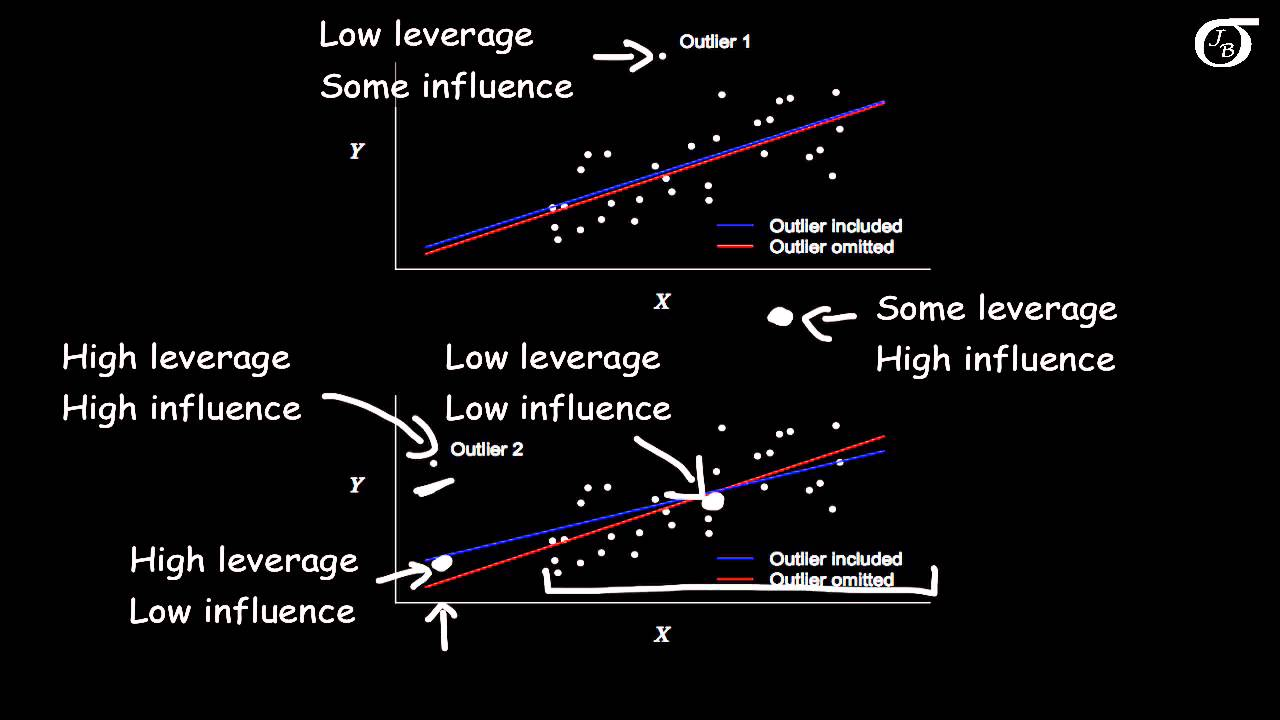
\includegraphics[width=\linewidth]{lev}
\end{center}
\caption{leverage and influence - {\small image by bj statistics} }

\label{fig:figure1}
\end{figure}

\section{Hat values}
The {\bf leverage} (Hat value) define how far apart is a given data point from the average(mean/median). It gauge the influence of the observed value of the outcome variable over the predicted values. Points with high leverage tend to pull the regression line toward themselves and have impact on the slop of the regression line hence {\bf influential}.

The {\bf average leverage} value is defined as $$\bar{h}=\frac{(k+1)}{n}$$ in which $k$ is the number of predictors in the model and $n$ is the number of participants.

{\bf Hat-matrix}  

\bigskip
The algebraic expression of linear regression.
$$\hat{y} = Hy$$
Where:\\
$\hat{y}$ is the prediction from the full regression model for observation; \\
$H = X(X^tX)^{-1}X^t$ is the $n$x$n$  prediction matrix also called hat matrix because it maps $y$ into the fitted $\hat{y}$\\
The information of the influence of $y_i$ on the fit of the model is contained in $h_{ii}$, the corresponding diagonal element in the hat matrix.\\ 

$$ h_{ii} = \frac{\partial{\hat{y}_i}}{\partial y_i}$$
where $\hat{y}_i$ and ${y}_i$ are the fitted and measured observation, respectively.
$$ h_{ii} =\frac{1}{n} + \frac{(X_i - \bar{X}_i)^2 }{\sum(X_i - \bar{X}_i)^2}$$

\section{Interpretation }

In {\bf simple regression}, Leverage is the proportion of the total sum of squares of the explanatory variable contributed by the $ith$ case.

In{ \bf multiple regression} (several x variable),hat value is represented as $$h_ii = (H)_{ii}$$
Where $H$ is the hat matrix.
\bigskip
Leverage values can lie between 0 (indicating that the case has no influence whatsoever) and 1 (indicating that the case has complete influence over prediction). If no cases exert undue influence over the model then we would expect all of the leverage values to be close to the average value $((k + 1)/n)$. Hoaglin and Welsch (1978) recommend investigating cases with values greater than twice the average$ (2(k + 1)/n)$ and Stevens (2002) recommends using three times the average $(3(k + 1)/n)$ as a cut-off point for identifying cases having undue influence.\citep{DSUR}
\section{Hat value using R}
In this example we use album sales2 data from the book "Discovering Statistics Using R" \citep{DSUR} \\
First we build the fitted regression model after loading the data \\
\texttt{album2<-read.delim("Album Sales 2.dat", header = TRUE)\\
\# run the multiple regression model\\
lm\_model<-lm(sales ~ adverts + airplay + attract, data = album2)\\
\# analyse hat values by calling the built-in function hatvalue()\\
hat\_v <- hatvalues(lm\_moldel)\\
\# determine influential points by applying the threshold of 3*average(hat value)\\
Average hat value : (k+1)/n\\
\# result [1]:0.02\\
influential\_hat <- hat\_v > 3*0.02\\
we managed to isolate points at positions 7, 12, 138, 181, 184}\\
Now we plot the hat values \\
\texttt{plot(hat\_v, ylab = "hat values")\\
\# point with exceptional hat value will be shown green\\ 
points(7,hat\_v[7], col = 'green')\\
points(12, hat\_v[12], col = 'green')\\
points(138, hat\_v[138], col = 'green')\\
points(181, hat\_v[181], col = 'green')\\
points(184, hat\_v[184], col = 'green')}

\begin{figure}[h]
\begin{center}
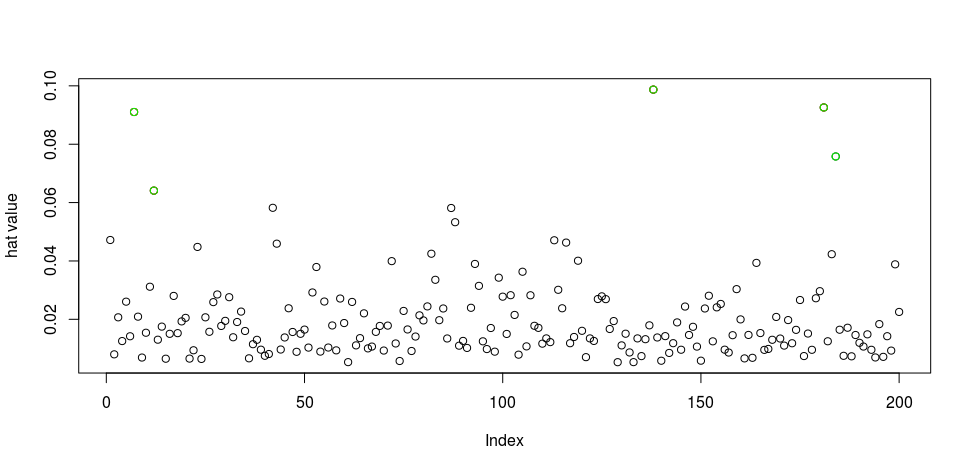
\includegraphics[width=\linewidth]{hat_v}
\end{center}
\caption{Hat values on 200 album sales data}

\label{fig:figure1}
\end{figure}

\newpage

\section{Discussion}
{ \bf What should we do when a given data-point's $ \hat{y} > threshold$ ?:}\\


First we should make sure that the observation is recorded correctly\\
Do the outcome change when the data is removed from the calculation? if the outcome do not change, it's not a big deal, but if the outcome change then this a problem that we need to fix. We don't want our statistical model relaying on a single data-point.\\

In that case we could reports two different results , one whit the influential data and another one without the the influential data.\\

Or we could restrict the analysis to values of $X$ for which the relationship holds. Which is usually not a good idea since we are omitting a data-point even though we would report that a outlier has been removed from the calculation. 



\bigskip


\bibliographystyle{ACM}
\bibliography{Hat_value}
\end{document}